\documentclass{article}
\usepackage{graphicx}
\usepackage{subfig}
\usepackage{url}


\title{Problem Statement: Creating Provenance from System Call Traces}

\begin{document}
\maketitle

\begin{abstract}
This document gives a high level overview of the research project and its goals, as well as details on the inputs and expected end result.
\end{abstract}

\section{The research project}
Science is the art of coming up with questions and their answers, so it's always good to start with the questions. Obviously, there are lots of things we can do with the data, but here are a few things I'm trying to figure out.
\begin{enumerate}
\item Given a provenance graph, can we accurately predict what file people will access next?
\item In particular, can we figure out what ONE person will access next? (Personalized prediction)
\item Can we identify some characteristics of file access that are unique to bioinformatics?
\end{enumerate}

What we have right now is a bunch of long term system call traces from systems that have been used for computer science research, and a bioinformatics cluster that hasn't been installed yet. So we're focusing on turning the traces we have into a graph, and then once the cluster comes up, we can worry about getting traces from it. (Also, if we run into snags with the traces we have, we can avoid wasting time later)

\section{The data}
The data we're working with is from the LASR system.  It will look something like the following:
\begin{verbatim}
0 RESTART (scratch) at 1008288727 Thu Dec 13 19:12:07 2001
32 UID 0 PID 812 ?? B 1008288727.376532 execve("/sbin/syslogd") = 0
76 UID 0 PID 812 /sbin/syslogd A 1008288727.437433 execve("") = 0
104 UID 0 PID 812 /sbin/syslogd A 1008288727.437576 open("/etc/ld.so.preload", O_RDONLY, 0) = -1 (2)
160 UID 0 PID 812 /sbin/syslogd A 1008288727.437633 open("/etc/ld.so.cache", O_RDONLY, 78748) = 3
216 UID 0 PID 812 /sbin/syslogd B 1008288727.437650 close(3, 78748) = 0
252 UID 0 PID 812 /sbin/syslogd A 1008288727.437706 open("/lib/i686/libc.so.6", O_RDONLY, 5772268) = 3
308 UID 0 PID 812 /sbin/syslogd A 1008288727.437723 read(3, 1024) = 1024
344 UID 0 PID 812 /sbin/syslogd B 1008288727.437844 close(3, 5772268) = 0
380 UID 0 PID 812 /sbin/syslogd A 1008288727.439369 chdir("/") = 0
412 UID 0 PID 812 /sbin/syslogd A 1008288727.439558 open("/var/run/syslogd.pid", O_RDONLY, 0) = -1 (2)
472 UID 0 PID 813 /sbin/syslogd A 1008288727.439762 fork(812) = 0
504 UID 0 PID 813 /sbin/syslogd A 1008288727.442123 open("/var/run/syslogd.pid", O_RDONLY, 0) = -1 (2)
564 UID 0 PID 813 /sbin/syslogd A 1008288727.442205 open("/var/run/syslogd.pid", O_CREAT|O_RDWR, 0) = 0
624 UID 0 PID 813 /sbin/syslogd A 1008288727.442593 write(0, 4) = 4
660 UID 0 PID 813 /sbin/syslogd B 1008288727.442605 close(0, 4) = 0
696 UID 0 PID 813 /sbin/syslogd A 1008288727.442911 open("/etc/resolv.conf", O_RDONLY, 94) = 0
752 UID 0 PID 813 /sbin/syslogd A 1008288727.443008 read(0, 4096) = 94
788 UID 0 PID 813 /sbin/syslogd A 1008288727.443057 read(0, 4096) = 0
824 UID 0 PID 813 /sbin/syslogd B 1008288727.443077 close(0, 94) = 0
860 UID 0 PID 813 /sbin/syslogd A 1008288727.443280 open("/etc/nsswitch.conf", O_RDONLY, 1750) = 0
916 UID 0 PID 813 /sbin/syslogd A 1008288727.443333 read(0, 4096) = 1750
952 UID 0 PID 813 /sbin/syslogd A 1008288727.443468 read(0, 4096) = 0
\end{verbatim}

It's kind of obtuse, but you can see that there's a uid and a pid (user and process). There's a UNIX time stamp (like 962559821.223242), a system call name (like unlink), and then some arguments, and a return value.
\section{Provenance graphs}
A provenance graph has nodes, edges, and ``annotations" (basically extra info). There are two kinds of nodes, processes and files. Edges connect files to processes, or vice versa, and are directed in order of dependency. So, for instance, if a process opens a file and reads it, then the edge goes from the process to the file, because the process ``depends" on the file (See Figure \ref {fig:read}). For a write, the edge goes the other way, from the file to the process (Figure \ref{fig:write}). If a process starts another process, then the child depends on the parent, so the edge goes from the child process to the parent process (Figure \ref{fig:spawnreadwrite}).
%USE SUBFIGURE
%\begin{figure}[h!]
%\subfloat[Process reads file][Process reads file]{
%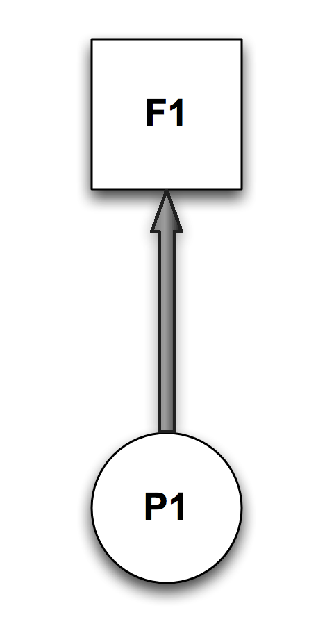
\includegraphics[width=0.25\textwidth]{figs/readfile}
%\label{fig:subfig1}}

%
%\subfloat[Process writes file][Process writes file]{
%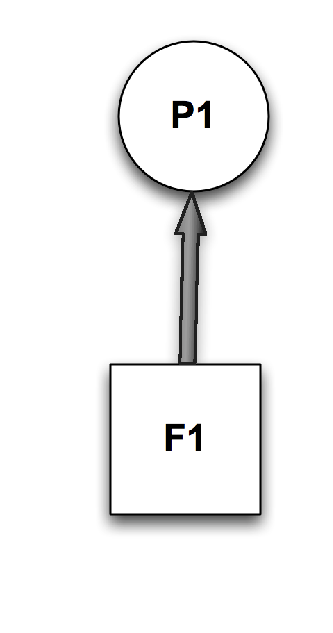
\includegraphics[width=0.25\textwidth]{figs/writefile}
%\label{fig:subfig2}}

%
%\subfloat[Process starts another process which reads one file, and then writes another.][Process starts another process which reads one file, and then writes another.]{
%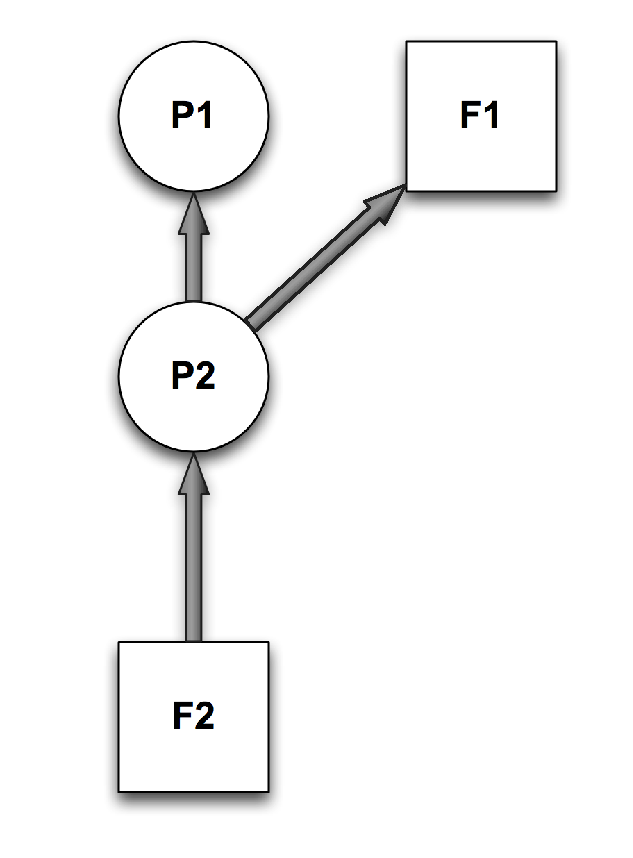
\includegraphics[width=0.25\textwidth]{figs/spawnreadwrite}
%\label{fig:subfig3}}
%\end{figure}

\begin{figure}[h!]
  \centering
    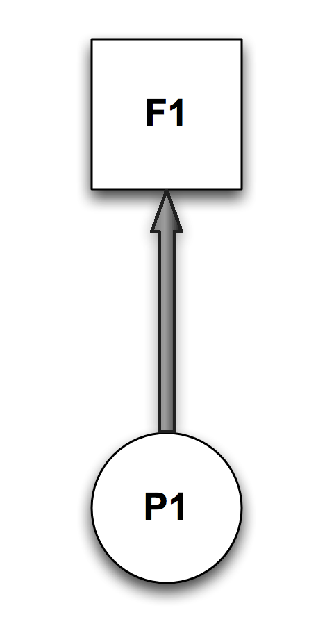
\includegraphics[width=.25\textwidth]{figs/readfile}
      \caption{Process reads file.}
      \label{fig:read}
\end{figure}

\begin{figure}[h!]
  \centering
    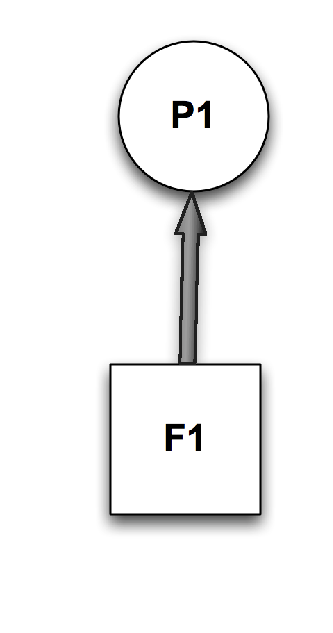
\includegraphics[width=.25\textwidth]{figs/writefile}
      \caption{Process writes file.}
      \label{fig:write}
\end{figure}


\begin{figure}[h!]
  \centering
    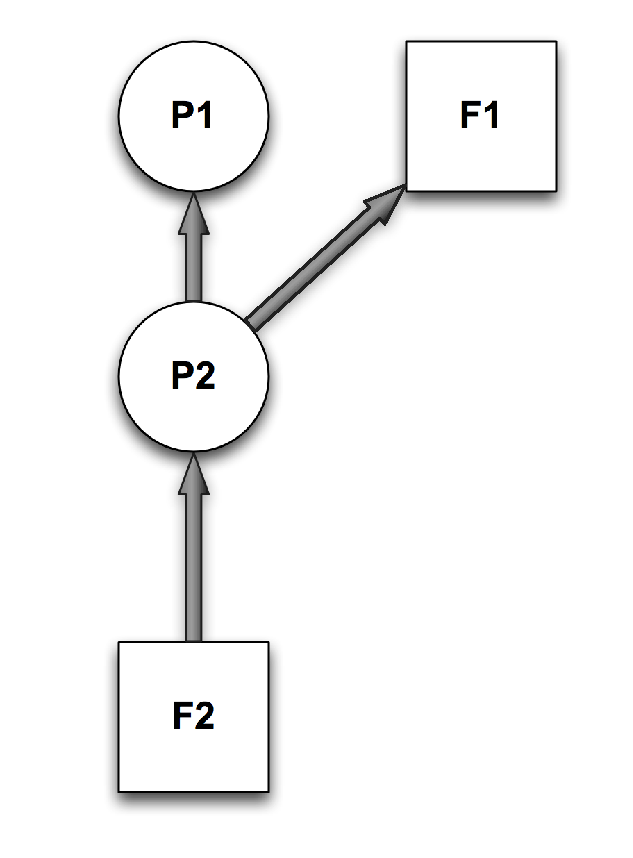
\includegraphics[width=.25\textwidth]{figs/spawnreadwrite}
      \caption{Process starts another process which reads one file, and then writes another.}
      \label{fig:spawnreadwrite}
\end{figure}

However, that's not quite as much information as we need for full causality. So we add annotations, in the form of users, time stamps, and versions.  (We'll also add in the name of the executable for each file.) When a file is changed, we declare that to be a new version of that file, so we might have results.txt(v1), results.txt(v2), etc. That way we can say which version of a file another file got data from, and we know which processes contributed up to that point.  (And it breaks cycles which would otherwise be very misleading.)  I have an example in Figure \ref{fig:cycle}.

\begin{figure}[h!]
  \centering
    \includegraphics[width=.4\textwidth]{figs/cycle}
      \caption{Process reads file.}
      \label{fig:cycle}
\end{figure}

\section{Actually generating the graph}
Figure \ref{fig:cycle} is the kind of graph we're going to be generating.  We'll take a list of system calls, and use it to figure out the dependency structure of files and processes. We'll infer the existence of processes based on their fork and exec calls, and then use their opens, closes, reads, and writes to infer the existence of files.  We'll annotate every process with the name of its owner, and every time a file gets written, we'll create a new ``version" of that node in the graph.  Every edge in the graph will have a timestamp.

Process IDs are reused by the system, so we need to make sure we have a unique identifier for the process.  We'll use the \texttt{execve} timestamp (the beginning one, since we have both) to make a unique ID.

We are going to write the file out into a plain text format that's used by a program called \texttt{graphviz} (\url{http://www.graphviz.org/}), so we can look at it and sanity check it as we go.  Figure \ref{fig:gvcycle} is what Figure \ref{fig:cycle} would look like in graphviz format, and with more realistic process IDs and file names: 

\begin{verbatim}
digraph "unix" {
  rankdir=BT;
	graph [	fontname = "Helvetica-Oblique",
		fontsize = 36,
		label = "\n\n\n\nExample Provenance Graph",
		size = "6,6" ];
	node [	shape = rectangle,
		color = white,
		style = filled,
		fontname = "Helvetica-Outline" ];
	"PID470_1362438507.437433" [label = "PID470\n/bin/vi\nUser 1", color=darkolivegreen3];
	"~/test.txt" [label = "~/test.txt\nVersion 1", shape = circle, color=lightsteelblue1];
  "PID470_1362438507.437433" -> "~/test.txt" [label = "3/4/13 2:45 pm"];
  
  "~/test2.txt" [label = "~/test2.txt\nVersion 1", shape = circle, color=lightsteelblue1];
  "~/test2.txt" -> "PID470_1362438507.437433" [label = "3/4/13 2:47 pm"];
  
  "PID483_1362438687.437235" [label = "PID483\n/bin/cp\nUser 1", color=darkolivegreen3];
  "PID483_1362438687.437235" -> "~/test2.txt" [label = "3/4/13 2:48 pm"];
  
  "~/test.txtv2" [label = "~/test.txt\nVersion 2", shape = circle, color=lightsteelblue1];
  "~/test.txtv2" -> "PID483_1362438687.437235" [label = "3/4/13 2:50 pm"];
}
}
\end{verbatim}

\begin{figure}[h!]
  \centering
    \includegraphics[width=.4\textwidth]{figs/gvcycle}
      \caption{Graphviz diagram}
      \label{fig:gvcycle}
\end{figure}


\end{document}

